\documentclass[12pt,article]{article}
\usepackage{lmodern}
\usepackage{amssymb,amsmath}
\usepackage{ifxetex,ifluatex}
\usepackage{fixltx2e} % provides \textsubscript
\ifnum 0\ifxetex 1\fi\ifluatex 1\fi=0 % if pdftex
  \usepackage[T1]{fontenc}
  \usepackage[utf8]{inputenc}
\else % if luatex or xelatex
  \ifxetex
    \usepackage{mathspec}
    \usepackage{xltxtra,xunicode}
  \else
    \usepackage{fontspec}
  \fi
  \defaultfontfeatures{Mapping=tex-text,Scale=MatchLowercase}
  \newcommand{\euro}{€}
\fi
% use upquote if available, for straight quotes in verbatim environments
\IfFileExists{upquote.sty}{\usepackage{upquote}}{}
% use microtype if available
\IfFileExists{microtype.sty}{%
\usepackage{microtype}
\UseMicrotypeSet[protrusion]{basicmath} % disable protrusion for tt fonts
}{}
\usepackage[margin=1.25in]{geometry}
\ifxetex
  \usepackage[setpagesize=false, % page size defined by xetex
              unicode=false, % unicode breaks when used with xetex
              xetex]{hyperref}
\else
  \usepackage[unicode=true]{hyperref}
\fi
\hypersetup{breaklinks=true,
            bookmarks=true,
            pdfauthor={Justin Murphy},
            pdftitle={Does Public Support for UKIP Drive Media Coverage or Does Media Coverage Drive Support for UKIP?},
            colorlinks=true,
            citecolor=blue,
            urlcolor=blue,
            linkcolor=blue,
            pdfborder={0 0 0}}
\urlstyle{same}  % don't use monospace font for urls
\usepackage{graphicx,grffile}
\makeatletter
\def\maxwidth{\ifdim\Gin@nat@width>\linewidth\linewidth\else\Gin@nat@width\fi}
\def\maxheight{\ifdim\Gin@nat@height>\textheight\textheight\else\Gin@nat@height\fi}
\makeatother
% Scale images if necessary, so that they will not overflow the page
% margins by default, and it is still possible to overwrite the defaults
% using explicit options in \includegraphics[width, height, ...]{}
\setkeys{Gin}{width=\maxwidth,height=\maxheight,keepaspectratio}
\setlength{\parindent}{0pt}
\setlength{\parskip}{6pt plus 2pt minus 1pt}
\setlength{\emergencystretch}{3em}  % prevent overfull lines
\providecommand{\tightlist}{%
  \setlength{\itemsep}{0pt}\setlength{\parskip}{0pt}}
\setcounter{secnumdepth}{0}

%%% Use protect on footnotes to avoid problems with footnotes in titles
\let\rmarkdownfootnote\footnote%
\def\footnote{\protect\rmarkdownfootnote}

%%% Change title format to be more compact
\usepackage{titling}

% Create subtitle command for use in maketitle
\newcommand{\subtitle}[1]{
  \posttitle{
    \begin{center}\large#1\end{center}
    }
}

\setlength{\droptitle}{-2em}
  \title{Does Public Support for UKIP Drive Media Coverage or Does Media Coverage
Drive Support for UKIP?}
  \pretitle{\vspace{\droptitle}\centering\huge}
  \posttitle{\par}
  \author{Justin Murphy}
  \preauthor{\centering\large\emph}
  \postauthor{\par}
  \date{}
  \predate{}\postdate{}

\usepackage{dcolumn}
\usepackage{setspace}

% Redefines (sub)paragraphs to behave more like sections
\ifx\paragraph\undefined\else
\let\oldparagraph\paragraph
\renewcommand{\paragraph}[1]{\oldparagraph{#1}\mbox{}}
\fi
\ifx\subparagraph\undefined\else
\let\oldsubparagraph\subparagraph
\renewcommand{\subparagraph}[1]{\oldsubparagraph{#1}\mbox{}}
\fi

\begin{document}
\maketitle

\begin{abstract}
Previous research suggests media attention may cause support for populist right-wing parties, but this finding is debated and extant evidence remains limited to proportional representation systems in which such an effect would be most likely. At the same time, in the United Kingdom's first-past-the-post system, an ongoing political and regulatory debate revolves around whether the media give disproportionate coverage to the populist right-wing UK Independence Party (UKIP). Thus, we use a mixed-methods approach to investigate the causal dynamics of UKIP support and media coverage as an especially valuable case. Vector autoregression (VAR) using monthly, aggregate time-series data from 2004 to September 2015 provides additional evidence, from a new and less-likely institutional environment, consistent with the model that media drive party support, but not vice-versa. Additionally, qualitative investigation of
the dynamics suggests that in at least two key periods of stagnating or declining support for UKIP, media coverage increased and was followed by increases in public support. Overall the findings show that media coverage can and does
appear to drive public support in a substantively important fashion irreducible
to previous levels of public support.
\end{abstract}
\doublespacing

\section{Introduction}\label{introduction}

If the visibility of a political party in the media shapes the public
support it receives, then the degree to which the media gives attention
to different political parties can have significant implications for
democracy. In the United Kingdom, critics allege that the media pays
disproportionate attention to the populist, right-wing UK Independence
Party (UKIP) but media elites claim that media coverage of UKIP is
driven by increasing public support for the party. Descriptively, media
attention to UKIP is greater than that given to other, similarly sized
parties on the right as well as the left (Goodwin and Ford, 2013;
Stevenson, 2014; Soussi, 2014), but UK media regulator Ofcom as well as
the BBC have publicly defended the attention paid to UKIP on grounds of
public support for the party (Sweeney, 2015; Wintour, 2015). Implied in
this elite reasoning is a causal model, namely that public support
drives media coverage rather than vice-versa.

Yet previous research from proportional representation systems suggests
that public support does not drive media coverage for populist
right-wing parties, but rather their media coverage drives their public
support (Boomgaarden and Vliegenthart, 2007, 2009; Vliegenthart et al.,
2012). By leveraging this insight to examine the dynamics of UKIP
support and media coverage, we fill an important gap in current research
on the visibility-support nexus while directly addressing a pressing
political research question (Dan: Can you find a citation(s) in a good
UK politics journal calling more policy/impact-driven research agendas?)
First, we contribute to current research on the visibility-support nexus
by testing a key insight from this research in a new institutional
context where hypothesized relationship should be less likely. Because
proportional representation systems are associated with a greater number
of small parties (Downs) and they tend to produce more diverse news
(Benson, 2009; Sheafer and Wolfsfeld, 2009; Kumlin, 2001; Strömbäck and
Dimitrova, 2006; Baum, 2012), research confined to such systems is
arguably most likely to reflect a model in which media coverage
generates support for populist right-wing parties. In a
first-past-the-post system where we typically expect only two parties
and media to be less diverse, these institutional pressures make it more
difficult for the media to generate support for smaller populist,
right-wing parties. Thus, testing this theory with time-series data from
a first-past-the-post system contributes to either refining the scope
conditions of previous research (in the case of unexpected findings) or
else extending and strengthening our confidence in the media-support
dynamic. Additionally, we make contribute to a pressing regulatory
question in UK national politics, as the democratic quality of UK media
regulation with respect to political party favouritism, especially
regarding populist right-wing parties, remains on public trial. This
article lends insight into the causal dynamics usually implied in such
political debates.

\pagebreak

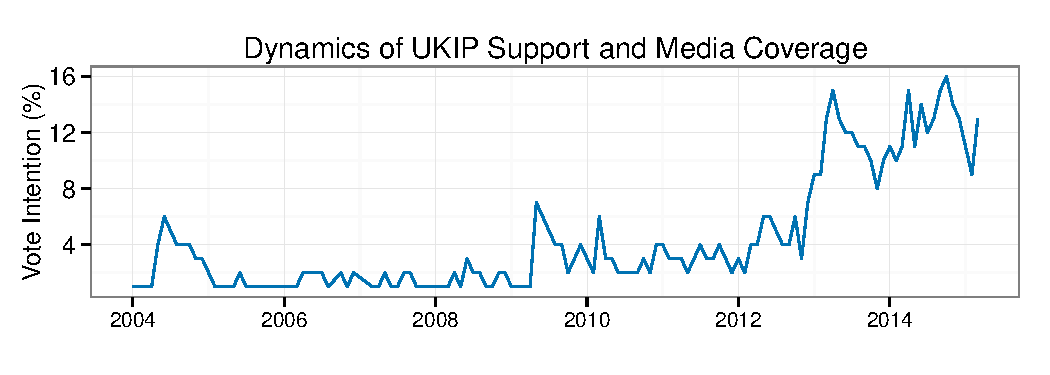
\includegraphics{ukip_media_files/figure-latex/unnamed-chunk-1-1.pdf}
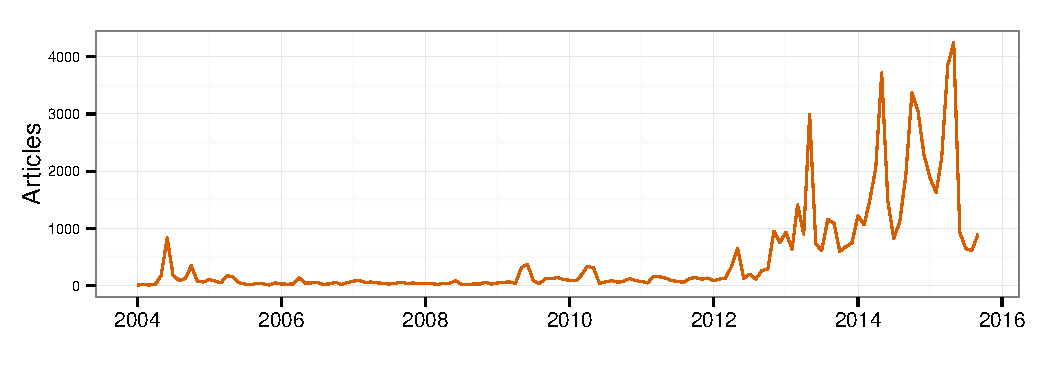
\includegraphics{ukip_media_files/figure-latex/unnamed-chunk-1-2.pdf}

\begin{figure}[htbp]
\centering
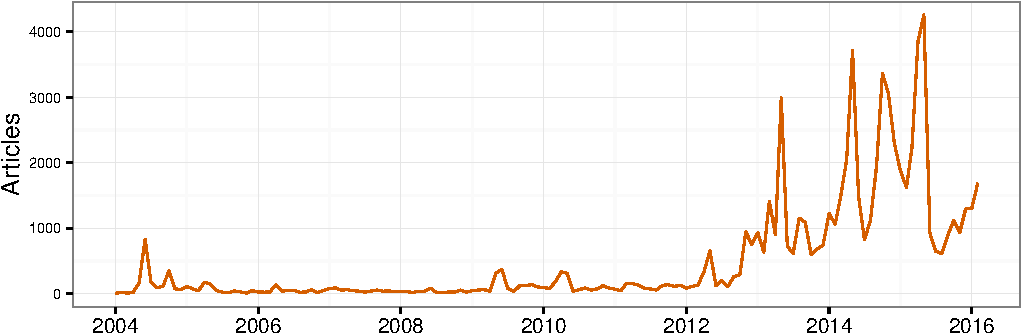
\includegraphics{ukip_media_files/figure-latex/unnamed-chunk-2-1.pdf}
\caption{Dynamics of UKIP Support and Media Coverage}
\end{figure}

\section{Theory}\label{theory}

A large body of research suggests that mass media coverage, as the
primary channel through which the electorate receives information about
politicians and parties, affects many different aspects of electoral
politics (Norris, 2000; Paletz, 1996; Beck et al., 2002; Dalton et al.,
1998). If media coverage of political parties is driven by public
support for the parties--even if media coverage then increases public
support further--it could be argued that media are facilitating popular
sovereignty. On the other hand, if media coverage independently changes
public support rather than reflects it, this would represent a point of
crucial possible distortion in the functioning of a democracy. The
latent normative motivation for the present investigation is whether the
quantity of UKIP's media coverage represents a form of media bias which
produces rather than reflects public opinion, or if the media's
fascination with UKIP is a democratically appropriate response to a
rising dimension of public opinion.

Previous research on the dynamics of media coverage and party support is
consistent with the argument that quantity of media coverage drives
party support in Belgium (WALGRAVE and SWERT, 2004), the Netherlands,
and Germany (Boomgaarden and Vliegenthart, 2007, 2009; Vliegenthart and
Boomgaarden, 2010; Vliegenthart et al., 2012). At the individual level,
panel data from the Netherlands suggests that media coverage drives
perceptions of right-wing populist politicians as well as mainstream
politicians (Bos et al., 2011). At the level of electoral results,
(Hopmann et al., 2010) showed that media coverage was one of the best
predictors of electoral success in the 2007 Dutch election. (Koopmans
and Muis, 2009) showed that in the Netherlands, media coverage of
Fortuyn improved polling performance before the 2002 election. Media
coverage has also been found to help explain party preferences in
Germany (Semetko and Schoenbach, 1994) and the Netherlands (Oegema and
Kleinnijenhuis, 2009).

Other scholars have addressed the question indirectly. In his study on
the diffusion of the populist message in the media, (Rooduijn, 2014)
hypothesises that the electoral success of populist parties affects the
degree and acceptability of populism in the media. Other authors in the
literature explore the theoretical connection between media coverage and
the rise of populist and right-wing parties, but offer little or no
empirical evidence for the claim (Art, 2007; Mudde, 2013). Nevertheless,
there is a considerable body of literature which posits particular
mechanisms which may offer a causal explanation for how the quantity of
media coverage can increase support for a political party. The primary
explanation revolves around issue saliency and the aligning of a party
or a party leader with those salient issues (Brug et al., 2006; Cushion
et al., 2015; Dennison and Goodwin, 2015). In the case of UKIP, the
party was strongly aligned with the issue of immigration and the
European Union, and the increasing prominence of these issues in the
media may have driven both coverage and support for the party. (WALGRAVE
and SWERT, 2004) offer a similar analysis of the Vlaams Blok in Belgium,
concluding that the media are at least part responsible for the growth
of the right-wing party. Although that study does conclude in support of
this relationship, they do not commit themselves to arguing a causal
relationship.Thus we test the hypothesis that:

is based on data from proportional representation (PR) electoral
systems.

although some have called these findings into question on the basis of
methodological concerns (Pauwels, 2010).

In part, this may be because the application of time-series techniques
to aggregate media data remains relatively under-explored (Vliegenthart,
2014).

H1: Increases in media coverage lead to increased public support,
controlling for previous levels of public support.

It is also theoretically plausible that changes in public support for
party receives may lead to changes in media coverage. As (Vliegenthart
and Boomgaarden, 2010) consider, this could be related to the power and
position of political figures, referencing studies from both America
(Sellers and Schaffner, 2007) and Switzerland (Tresch, 2009) which
highlight how the standing of a political actor influences media
attention. Another possibility is that media coverage depends on the
dynamics of the party itself (Pauwels, 2010): in our case, the relative
acceptability of UKIP's agenda as opposed to other British populist
parties such as the British National Party may have contributed to the
rise in coverage, as well as the popularity and charisma of Nigel
Farage. Finally, political polling and the reporting of political polls
is ubiquitous in British media, including tabloid papers running polls
of their own readers. It could be the case that increasing media
coverage is simply reflective of their standing in polls, or that there
is a positive feedback mechanism operating between media coverage and
polling. We therefore test this possibility, hypothesising that:

H2: Increases in public support for UKIP lead to increased media
coverage, controlling for previous levels of media coverage

\section{Data, Method, and Research
Strategy}\label{data-method-and-research-strategy}

To measure public support for UKIP, we gathered monthly aggregate
polling data on vote intentions from Ipsos MORI (Ipsos-MORI, n.d.).
Specifically, we constructed a variable from the percentage reporting an
intention to vote for UKIP according to the Ipsos MORI poll closest to
the middle of each month. For most months, this was straightforward
because the Ipsos MORI poll is approximately monthly. For months with
multiple polls, we used the poll closest to the middle of the month. For
the very few months with no poll or a poll at the border between the
previous or following month, the value was counted as missing and then
all missing values were linearly interpolated. To measure media coverage
of UKIP, I gathered monthly counts of all UK national newspaper reports
mentioning either ``UKIP'' or ``UK Independence Party'' from the
database
Nexis.\footnote{Duplicate articles defined by Nexis's definition of high similarity were excluded.}

There is also reason to believe that elections themselves have an
independent effect on coverage and support due to general increased
media attention and through the running of public campaigns. For this
reason, we have included dummy variables for each national and European
election covered by the data. The elections included are three European
elections (2004, 2009 and 2014) and three general elections (2005, 2010
and 2015). Usefully, the European elections coincide with local
elections in the UK.

Econometric techniques are used to test for, and distinguish the
ordering of, potential causal dynamics between media coverage and public
support for UKIP. A brief qualitative historical analysis of these
dynamics will be used to better understand a potential causal process.
In particular, the substantive nature of the puzzle at hand requires the
identification of a causal narrative. Even with econometric evidence
suggesting an independent causal effect from either one to the other, it
would not be clear whether the historical unfolding of these causal
dynamics implies a problem for democracy. We are not only interested in
whether media coverage amplifies exogenous increases in support--this
would be an important but not necessarily problematic finding from a
democratic perspective--but whether increases in media coverage have
generated support for UKIP despite low, stagnant, or decreasing levels
of support.

\section{Analysis}\label{analysis}

\subsection{VAR}\label{var}

Because both variables are non-stationary, vector autoregression is
estimated with first differences of each variable. Optimal lag length is
determined by the Aikeke Information Criterion to be to be VAR(3). The
model includes a constant and a trend term. Diagnostics suggest that
using the log of each variable before differencing reduces
heteroskedasticity and serial correlation of errors. Because VAR models
have many paramaters to begin with, monthly indicators controlling for
seasonality absorb crucial degrees of freedom and so are excluded in the
intitial models but added in subsequent models. The models displayed
here all pass the standard ARCH-LM and Portmanteau tests for
non-constant error variance and serial correlation of errors,
respectively. Finally, diagnostics show no evidence of significant
temporal instability (see Supplementary Information).

Surprisingly, initial VAR results show little evidence that changes in
public support predict media coverage, but significant evidence that
media coverage drives public support. As the numerical results and the
Impulse Response plots show, there is no statistically discernable
correlation between past changes in public support and changes in media
coverage, whereas past changes in media coverage have a statistically
significant correlation with changes in public support. Granger
causality tests support this interpretation, with only the latter
relationship nearing conventional cutoffs of statistical significance
(p\textless{}.08).

After including monthly indicators, however, the results reverse: while
the coefficients reflecting the correlation between past changes in
media coverage and public support do not change noticeably, they lose
statistical significance, whereas the coefficients for the other model
become significant and pass the test for Granger causality. Because the
coefficients reflecting the correlation between past changes in media
coverage and public support remain signed as predicted, the increased
standard errors do not necessarily reflect the absence of a relationship
but possibly only a lack of degrees of freedom due to the introduction
of the seasonality indicators.

Additionally, there are limitations of the data which may make it
difficult to identify causal effects in a VAR approach. First, it is
possible that monthly measures are too infrequent to capture causal
effects if the real lag between effects is more shorter than one month.
Importantly, structural tests on all models suggest strong evidence of
instantaneous causality.

Taken together, VAR results suggest qualified evidence for both
directions of causality. While the results are sensitive to the
specification, the results are consistent with the possibility that both
variables drive each other, but that highly robust evidence of this in
one model is not possible due to the nature of the data and the
high-paramater demands of the VAR approach. \pagebreak

\% Table created by stargazer v.5.2 by Marek Hlavac, Harvard University.
E-mail: hlavac at fas.harvard.edu \% Date and time: Tue, Oct 27, 2015 -
19:40:34

\begin{table}[!htbp] \centering 
  \caption{} 
  \label{} 
\begin{tabular}{@{\extracolsep{5pt}}lcc} 
\\[-1.8ex]\hline 
\hline \\[-1.8ex] 
 & \multicolumn{2}{c}{\textit{Dependent variable:}} \\ 
\cline{2-3} 
\\[-1.8ex] & \multicolumn{2}{c}{y} \\ 
\\[-1.8ex] & (1) & (2)\\ 
\hline \\[-1.8ex] 
 UKIP.Articles.l1 & 0.168$^{*}$ & $-$0.387$^{***}$ \\ 
  & (0.095) & (0.094) \\ 
  & & \\ 
 UKIP.Vote.l1 & $-$0.483$^{***}$ & $-$0.007 \\ 
  & (0.106) & (0.105) \\ 
  & & \\ 
 UKIP.Articles.l2 & 0.160$^{*}$ & $-$0.341$^{***}$ \\ 
  & (0.093) & (0.092) \\ 
  & & \\ 
 UKIP.Vote.l2 & $-$0.261$^{**}$ & $-$0.085 \\ 
  & (0.103) & (0.102) \\ 
  & & \\ 
 UKIP.Articles.l3 & 0.161$^{*}$ & $-$0.196$^{**}$ \\ 
  & (0.091) & (0.090) \\ 
  & & \\ 
 UKIP.Vote.l3 & $-$0.111 & $-$0.088 \\ 
  & (0.096) & (0.096) \\ 
  & & \\ 
 const & 0.012 & 0.027 \\ 
  & (0.080) & (0.079) \\ 
  & & \\ 
 trend & 0.00000 & $-$0.0002 \\ 
  & (0.001) & (0.001) \\ 
  & & \\ 
 General.Elections & $-$0.099 & 0.185 \\ 
  & (0.273) & (0.271) \\ 
  & & \\ 
 EU.Elections & 0.465 & 0.894$^{***}$ \\ 
  & (0.296) & (0.294) \\ 
  & & \\ 
\hline \\[-1.8ex] 
Observations & 137 & 137 \\ 
R$^{2}$ & 0.148 & 0.233 \\ 
Adjusted R$^{2}$ & 0.087 & 0.179 \\ 
Residual Std. Error (df = 127) & 0.445 & 0.443 \\ 
F Statistic (df = 9; 127) & 2.448$^{**}$ & 4.284$^{***}$ \\ 
\hline 
\hline \\[-1.8ex] 
\textit{Note:}  & \multicolumn{2}{r}{$^{*}$p$<$0.1; $^{**}$p$<$0.05; $^{***}$p$<$0.01} \\ 
\end{tabular} 
\end{table}

\% Table created by stargazer v.5.2 by Marek Hlavac, Harvard University.
E-mail: hlavac at fas.harvard.edu \% Date and time: Tue, Oct 27, 2015 -
19:40:34

\begin{table}[!htbp] \centering 
  \caption{Granger Causality Tests} 
  \label{} 
\begin{tabular}{@{\extracolsep{5pt}} ccc} 
\\[-1.8ex]\hline \\[-1.8ex] 
 & Support & Articles \\ 
\hline \\[-1.8ex] 
P-value & $0.750$ & $0.060$ \\ 
DF1 & $3$ & $3$ \\ 
DF2 & $254$ & $254$ \\ 
F-test & $0.405$ & $2.499$ \\ 
\hline \\[-1.8ex] 
\end{tabular} 
\end{table}

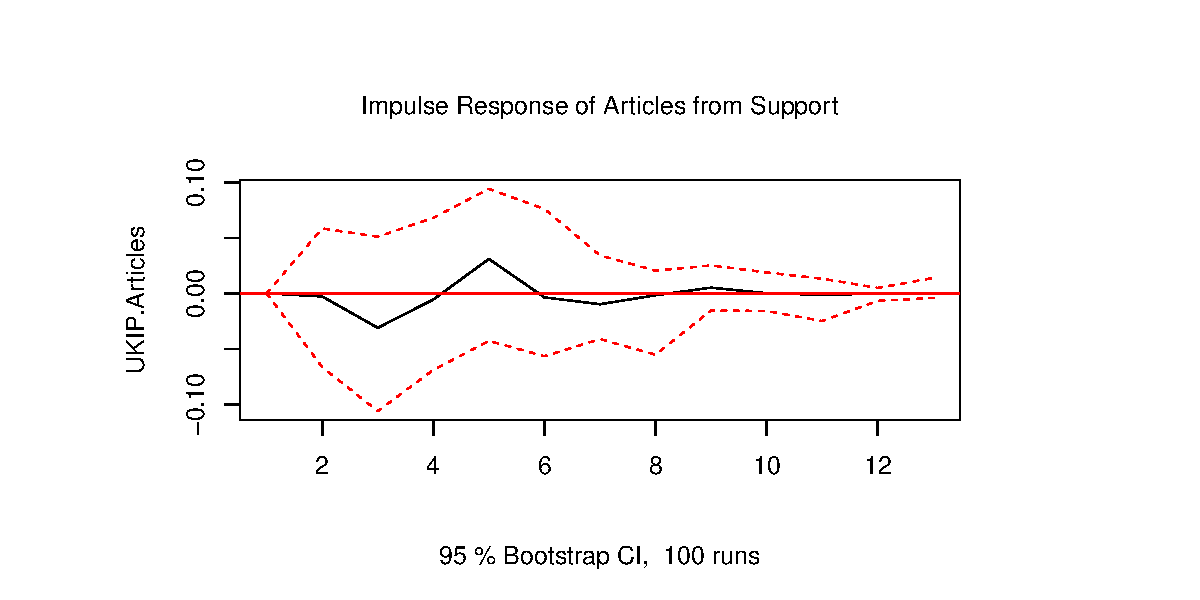
\includegraphics{ukip_media_files/figure-latex/unnamed-chunk-6-1.pdf}
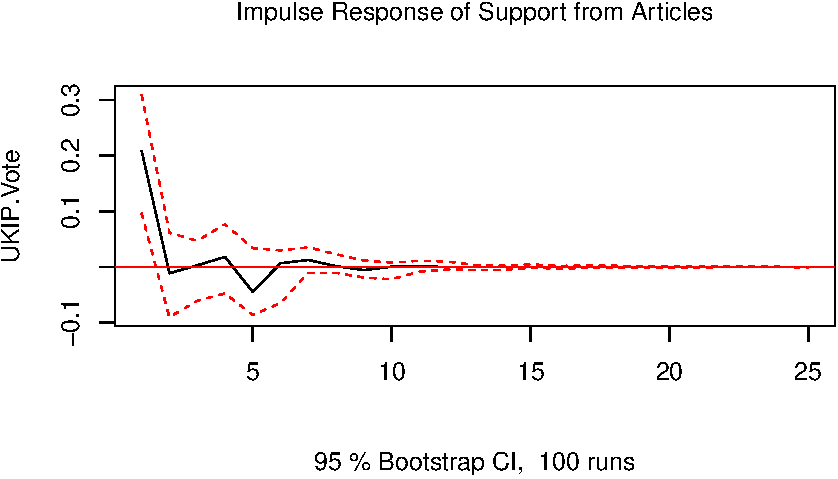
\includegraphics{ukip_media_files/figure-latex/unnamed-chunk-6-2.pdf}

\section{Process-tracing}\label{process-tracing}

This paper has investigated a simple claim by the UK’s regulatory
authorities and national broadcaster: that the increased media coverage
of UKIP was justified by the party’s increased poll ratings. We have
found that, on the contrary, on average media coverage preceded an
increase in poll ratings controlling for previous media coverage, rather
than media coverage increasing controlling for previous public support.
(Justin: perhaps write some results up from the models?).

\section{Conclusion}\label{conclusion}

We have made three contributions with this study. Firstly, this is the
first paper, in our knowledge, to address the visibility-support nexus
in the context of the United Kingdom and a majoritarian system; previous
research has primarily focused on other Western European democracies
such as Belgium, the Netherlands and Germany. Despite the change in
political system, our findings support those of (Vliegenthart and
Boomgaarden, 2010; Vliegenthart et al., 2012), and find that the media
can and have independently generated support for UKIP. We have left
aside the question of leader effects, given previously ambiguous
findings. There is also reason to believe that media dynamics are
different in proportional systems, being more diverse in their coverage
than in majoritarian systems.

Secondly, we have contributed methodologically in two ways. We have
offered qualitative evidence for our findings that, at least in this
case, the media have generated support for a radical right-wing party.
Previous research has offered only statistical evidence, which may not
pick up questions relating to the historical narrative of the party in
question. We address this gap here and find that the results are still
robust. We have also contributed to a growing body of literature that
uses time-series methods to address questions relating to the media
(Vliegenthart, 2014).

Perhaps most importantly, these findings are of significance to
contemporary public debate in the UK concerning the role of the media
and the perceived unfair coverage of UKIP. Some have argued that the
media coverage of UKIP is justified due to its public support. The
findings here, on the other hand, suggest that the causal arrow points
the other way: that the media coverage drove the support of UKIP
independent of its previous poll ratings.

As with all studies, there are limitations and areas for future
research. We do not undertake any form of content analysis to address
the actual content of the coverage in question, but only look at the
quantity of articles. It is possible that, by disaggregating the
coverage further, different types of coverage change the findings; it
would also be interesting to see whether how positive or negative the
coverage is matters for changing public opinion. Similarly, we do not
disaggregate between types of paper, such as broadsheet and tabloid,
which offer different coverage and target a different readership. We
also only focus on print media. This means that we have not accounted
for the effect of visual and social media which may be contributing to
this relationship. Despite these limitations, this paper provides a
contribution to the continuing and growing debate concerning the
media’s role in the growth of political parties and the wider
ramifications for democratic debate.

\pagebreak

\begin{figure}[htbp]
\centering
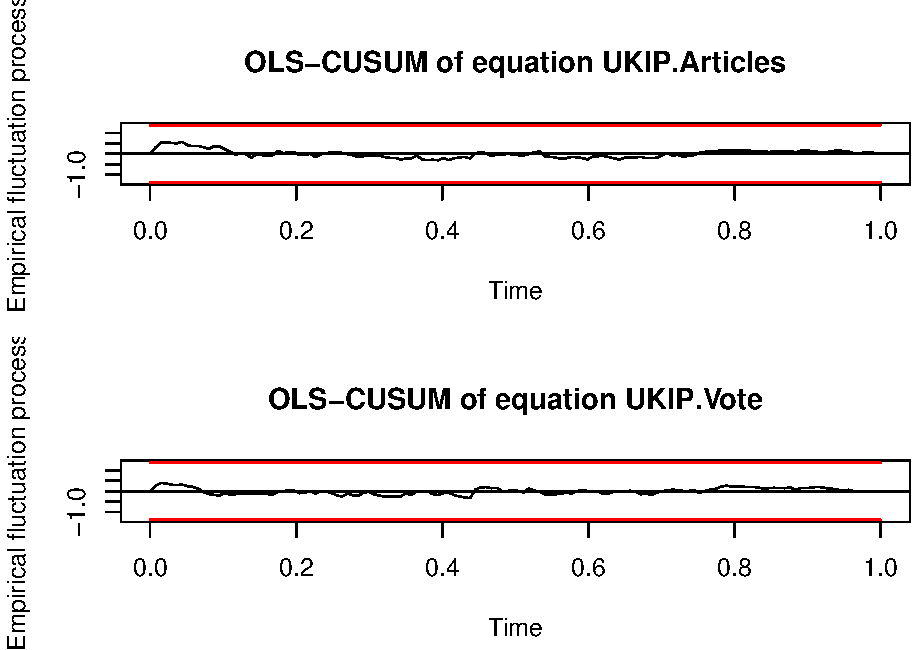
\includegraphics{ukip_media_files/figure-latex/supplementary-1.pdf}
\caption{}
\end{figure}

\pagebreak

\section{References}\label{references}

\raggedright

\hyperdef{}{ref-artux5freactingux5f2007}{\label{ref-artux5freactingux5f2007}}
Art, David. (2007) ``Reacting to the Radical Right Lessons from Germany
and Austria.'' \emph{Party Politics} 13:331--349.
\url{http://ppq.sagepub.com/content/13/3/331} (Accessed October 10,
2015).

\hyperdef{}{ref-Baum:2012je}{\label{ref-Baum:2012je}}
Baum, Matthew A. (2012) ``The Iraq Coalition of the Willing and
(Politically) Able: Party Systems, the Press, and Public Influence on
Foreign Policy.'' \emph{American Journal of Political Science}
57:442--458.

\hyperdef{}{ref-beckux5fsocialux5f2002}{\label{ref-beckux5fsocialux5f2002}}
Beck, Paul Allen, Russell J. Dalton, Steven Greene, and Robert
Huckfeldt. (2002) ``The Social Calculus of Voting: Interpersonal, Media,
and Organizational Influences on Presidential Choices.'' \emph{The
American Political Science Review} 96:57--73.
\url{http://www.jstor.org/stable/3117810} (Accessed October 26, 2015).

\hyperdef{}{ref-Benson:2009kb}{\label{ref-Benson:2009kb}}
Benson, Rodney. (2009) ``What makes news more multiperspectival? A field
analysis.'' \emph{Poetics} 37:402--418.
\url{http://linkinghub.elsevier.com/retrieve/pii/S0304422X09000412}.

\hyperdef{}{ref-Boomgaarden:2007ia}{\label{ref-Boomgaarden:2007ia}}
Boomgaarden, Hajo G, and Rens Vliegenthart. (2007) ``Explaining the rise
of anti-immigrant parties: The role of news media content.''
\emph{Electoral Studies} 26:404--417.

\hyperdef{}{ref-Boomgaarden:2009ke}{\label{ref-Boomgaarden:2009ke}}
Boomgaarden, Hajo G, and Rens Vliegenthart. (2009) ``How news content
influences anti-immigration attitudes: Germany, 19932005.''
\emph{European Journal of Political Research} 48:516--542.

\hyperdef{}{ref-Bos:2011iy}{\label{ref-Bos:2011iy}}
Bos, Linda, Wouter van der Brug, and Claes de Vreese. (2011) ``How the
Media Shape Perceptions of Right-Wing Populist Leaders.''
\emph{Political Communication} 28:182--206.

\hyperdef{}{ref-brugux5fmediaux5f2006}{\label{ref-brugux5fmediaux5f2006}}
Brug, Wouter van der, Holli A. Semetko, and Patti M. Valkenburg. (2006)
``Media Priming in a Multi-Party Context: A Controlled Naturalistic
Study in Political Communication.'' \emph{Political Behavior}
29:115--141.
\url{http://link.springer.com/article/10.1007/s11109-006-9020-7}
(Accessed October 3, 2015).

\hyperdef{}{ref-cushionux5finterpretingux5f2015}{\label{ref-cushionux5finterpretingux5f2015}}
Cushion, Stephen, Richard Thomas, and Oliver Ellis. (2015)
``Interpreting UKIP's `Earthquake' in British Politics: UK Television
News Coverage of the 2009 and 2014 EU Election Campaigns.'' \emph{The
Political Quarterly} 86:314--322.
\url{http://onlinelibrary.wiley.com/doi/10.1111/1467-923X.12169/abstract}
(Accessed October 1, 2015).

\hyperdef{}{ref-daltonux5fpartisanux5f1998}{\label{ref-daltonux5fpartisanux5f1998}}
Dalton, Russell J., Paul A. Beck, and Robert Huckfeldt. (1998)
``Partisan Cues and the Media: Information Flows in the 1992
Presidential Election.'' \emph{The American Political Science Review}
92:111--126. \url{http://www.jstor.org/stable/2585932} (Accessed October
3, 2015).

\hyperdef{}{ref-dennisonux5fimmigrationux5f2015}{\label{ref-dennisonux5fimmigrationux5f2015}}
Dennison, James, and Matthew Goodwin. (2015) ``Immigration, Issue
Ownership and the Rise of UKIP.'' \emph{Parliamentary Affairs}
68:168--187. \url{http://pa.oxfordjournals.org/content/68/suppl_1/168}
(Accessed October 1, 2015).

\hyperdef{}{ref-Goodwin:03LtHfhh}{\label{ref-Goodwin:03LtHfhh}}
Goodwin, Matthew, and Robert Ford. (2013) ``Just how much media coverage
does UKIP get?'' \emph{New Statesman}.
\url{http://www.newstatesman.com/politics/2013/11/just-how-much-media-coverage-does-ukip-get}.

\hyperdef{}{ref-hopmannux5feffectsux5f2010}{\label{ref-hopmannux5feffectsux5f2010}}
Hopmann, David Nicolas, Rens Vliegenthart, Claes De Vreese, and Erik
Albæk. (2010) ``Effects of Election News Coverage: How Visibility and
Tone Influence Party Choice.'' \emph{Political Communication}
27:389--405. \url{http://dx.doi.org/10.1080/10584609.2010.516798}
(Accessed October 10, 2015).

\hyperdef{}{ref-IpsosMORI:gm2fXYNK}{\label{ref-IpsosMORI:gm2fXYNK}}
Ipsos-MORI. (n.d.) ``Voting Intention in Great Britain: Recent Trends.''
\url{https://www.ipsos-mori.com/researchpublications/researcharchive/poll.aspx?oItemId=107\&view=wide}.

\hyperdef{}{ref-koopmansux5friseux5f2009}{\label{ref-koopmansux5friseux5f2009}}
Koopmans, Ruud, and Jasper Muis. (2009) ``The rise of right-wing
populist Pim Fortuyn in the Netherlands: A discursive opportunity
approach.'' \emph{European Journal of Political Research} 48:642--664.
\url{http://onlinelibrary.wiley.com/doi/10.1111/j.1475-6765.2009.00846.x/abstract}
(Accessed October 10, 2015).

\hyperdef{}{ref-Kumlin:2001iq}{\label{ref-Kumlin:2001iq}}
Kumlin, Staffan. (2001) ``IdeologyDriven opinion formation in Europe:
The case of attitudes towards the third sector in Sweden.''
\emph{European Journal of Political Research} 39:487--518.
\url{http://onlinelibrary.wiley.com.libproxy.temple.edu/doi/10.1111/1475-6765.00585/abstract}.

\hyperdef{}{ref-muddeux5fthreeux5f2013}{\label{ref-muddeux5fthreeux5f2013}}
Mudde, Cas. (2013) ``Three decades of populist radical right parties in
Western Europe: So what?'' \emph{European Journal of Political Research}
52:1--19.

\hyperdef{}{ref-norrisux5fvirtuousux5f2000}{\label{ref-norrisux5fvirtuousux5f2000}}
Norris, Pippa. 2000. \emph{A Virtuous Circle: Political Communications
in Postindustrial Societies}. Cambridge, UK: Cambridge University Press
\url{http://www.cambridge.org/gb/academic/subjects/politics-international-relations/comparative-politics/virtuous-circle-political-communications-postindustrial-societies}.

\hyperdef{}{ref-oegemaux5fpersonalizationux5f2009}{\label{ref-oegemaux5fpersonalizationux5f2009}}
Oegema, Dirk, and Jan Kleinnijenhuis. (2009) ``Personalization in
political Television News: A 13-Wave Survey Study to Assess Effects of
Text and Footage.'' \emph{Communications} 25:43--60.
\url{http://www.degruyter.com/view/j/comm.2000.25.issue-1/comm.2000.25.1.43/comm.2000.25.1.43.xml}
(Accessed October 26, 2015).

\hyperdef{}{ref-paletzux5fpoliticalux5f1996}{\label{ref-paletzux5fpoliticalux5f1996}}
Paletz, David. 1996. \emph{Political communication research: Vol. 2.
Approaches, studies, assessments}. Norwood, NJ: Ablex.

\hyperdef{}{ref-pauwelsux5freassessingux5f2010}{\label{ref-pauwelsux5freassessingux5f2010}}
Pauwels, Teun. (2010) ``Reassessing conceptualization, data and
causality: A critique of Boomgaarden and Vliegenthart's study on the
relationship between media and the rise of anti-immigrant parties.''
\emph{Electoral Studies} 29:269--275.
\url{http://www.sciencedirect.com/science/article/pii/S0261379410000120}
(Accessed October 10, 2015).

\hyperdef{}{ref-rooduijnux5fmesmerisingux5f2014}{\label{ref-rooduijnux5fmesmerisingux5f2014}}
Rooduijn, Matthijs. (2014) ``The Mesmerising Message: The Diffusion of
Populism in Public Debates in Western European Media.'' \emph{Political
Studies} 62:726--744.
\url{http://onlinelibrary.wiley.com/doi/10.1111/1467-9248.12074/abstract}
(Accessed October 2, 2015).

\hyperdef{}{ref-sellersux5fwinningux5f2007}{\label{ref-sellersux5fwinningux5f2007}}
Sellers, Patrick J., and Brian F. Schaffner. (2007) ``Winning Coverage
in the U.S. Senate.'' \emph{Political Communication} 24:377--391.
\url{http://dx.doi.org/10.1080/10584600701641516} (Accessed October 11,
2015).

\hyperdef{}{ref-semetkoux5fgermanysux5f1994}{\label{ref-semetkoux5fgermanysux5f1994}}
Semetko, Holli A, and Klaus Schoenbach. 1994. \emph{Germany's Unity
Election: Voters and the Media}. Cresskill: Hampton Press.

\hyperdef{}{ref-Sheafer:2009hi}{\label{ref-Sheafer:2009hi}}
Sheafer, Tamir, and Gadi Wolfsfeld. (2009) ``Party Systems and
Oppositional Voices in the News Media A Study of the Contest over
Political Waves in the United States and Israel.'' \emph{The
International Journal of Press/Politics} 14:146--165.
\url{http://hij.sagepub.com/cgi/doi/10.1177/1940161209333089}.

\hyperdef{}{ref-Soussi:vy}{\label{ref-Soussi:vy}}
Soussi, Alasdair. (2014) ``Did British media help the UKIP win EU
poll?''
\url{http://www.aljazeera.com/indepth/features/2014/06/did-british-media-help-ukip-win-eu-poll-20146313346918679.html}.

\hyperdef{}{ref-Stevenson:wo}{\label{ref-Stevenson:wo}}
Stevenson, Alex. (2014) ``Caroline Lucas points finger at media's Farage
obsession.''
\url{http://www.politics.co.uk/news/2014/05/29/ukip-victory-caroline-lucas-points-finger-at-media-s-farage}.

\hyperdef{}{ref-Stromback:2006ht}{\label{ref-Stromback:2006ht}}
Strömbäck, Jesper, and Daniela V Dimitrova. (2006) ``Political and Media
Systems Matter A Comparison of Election News Coverage in Sweden and the
United States.'' \emph{The International Journal of Press/Politics}
11:131--147.
\url{http://hij.sagepub.com.libproxy.temple.edu/content/11/4/131.abstract}.

\hyperdef{}{ref-Sweeney:wp}{\label{ref-Sweeney:wp}}
Sweeney, Mark. (2015) ``BBC prepares to boost Ukip coverage as it ranks
it a larger party in election.''
\url{http://www.theguardian.com/media/2015/jan/15/bbc-prepares-to-boost-ukip-coverage-as-it-ranks-it-a-larger-party-in-election}.

\hyperdef{}{ref-treschux5fpoliticiansux5f2009}{\label{ref-treschux5fpoliticiansux5f2009}}
Tresch, Anke. (2009) ``Politicians in the Media: Determinants of
Legislators' Presence and Prominence in Swiss Newspapers.'' \emph{The
International Journal of Press/Politics} 14:67--90.
\url{http://hij.sagepub.com/content/14/1/67} (Accessed October 11,
2015).

\hyperdef{}{ref-Vliegenthart:2014di}{\label{ref-Vliegenthart:2014di}}
Vliegenthart, Rens. (2014) ``Moving up. Applying aggregate level time
series analysis in the study of media coverage.'' \emph{Quality \&
Quantity} 48:2427--2445.

\hyperdef{}{ref-vliegenthartux5fwhyux5f2010}{\label{ref-vliegenthartux5fwhyux5f2010}}
Vliegenthart, Rens, and Hajo G. Boomgaarden. (2010) ``Why the media
matter after all: A response to Pauwels.'' \emph{Electoral Studies}
29:719--723.
\url{http://www.sciencedirect.com/science/article/pii/S0261379410000855}
(Accessed October 11, 2015).

\hyperdef{}{ref-vliegenthartux5fanti-immigrantux5f2012}{\label{ref-vliegenthartux5fanti-immigrantux5f2012}}
Vliegenthart, Rens, Hajo G. Boomgaarden, and Joost Van Spanje. (2012)
``Anti-Immigrant Party Support and Media Visibility: A Cross-Party,
Over-Time Perspective.'' \emph{Journal of Elections, Public Opinion and
Parties} 22:315--358.
\url{http://dx.doi.org/10.1080/17457289.2012.693933} (Accessed October
10, 2015).

\hyperdef{}{ref-walgraveux5fmakingux5f2004}{\label{ref-walgraveux5fmakingux5f2004}}
WALGRAVE, STEFAAN, and KNUT DE SWERT. (2004) ``The Making of the (Issues
of the) Vlaams Blok.'' \emph{Political Communication} 21:479--500.
\url{http://dx.doi.org/10.1080/10584600490522743} (Accessed October 10,
2015).

\hyperdef{}{ref-Wintour:vf}{\label{ref-Wintour:vf}}
Wintour, Patrick. (2015) ``Ofcom deals blow to Greens election debate
hopes but boosts Ukips.''
\url{http://www.theguardian.com/politics/2015/jan/08/ofcom-blow-green-party-election-debate-boost-ukips}.

\end{document}
